\documentclass{article}
\usepackage{graphicx}
\usepackage[utf8]{inputenc}
\usepackage{microtype}
\usepackage{graphicx}
\usepackage{subfigure}
\usepackage{booktabs}
\usepackage{hyperref}
\newcommand{\theHalgorithm}{\arabic{algorithm}}
\usepackage{icml2019}

\icmltitlerunning{Submission for ECE 570 Term Paper, Fall 2019}

\begin{document}

\twocolumn[
\icmltitle{ECE 570 Term Paper : A Review of
\\
Depth Estimation Algorithms Using Stereo Imaging}
\icmlsetsymbol{equal}{*}

\begin{icmlauthorlist}
\icmlauthor{Tyler Baumgartner}{}
\end{icmlauthorlist}

\vskip 0.0in
]

\begin{abstract}
The purpose of this paper is to review state-of-the-art methods for generating disparity maps between stereo images and to evaluate the effectiveness of using the notable PatchMatch algorithm \citep{barnes2009patchmatch} to efficiently estimate disparity between stereo images. When compared to the classic stereo algorithm approach of searching over all possible disparities, my algorithm implementing PatchMatch was able to greatly reduce runtime while maintaining a comparable error rate. More work needs to be done, however, to further refine this algorithm before it is tested against advanced CNN disparity estimating models such as DeepPruner \citep{duggal2019deeppruner}.
\end{abstract}

\section{Motivation and Problem Setting}
\label{motivation}
The ability to estimate absolute or relative depth based on stereo imagery is an ongoing issue that has ramifications in many fields such as autonomous vehicles, robotics, and image editing. Currently, most autonomous or semi-autonomous vehicles or robots rely on LiDAR, sonar, or other similar technologies to estimate depth for their environment, but these solutions often have a steep cost/performance tradeoff. Further, image and video editing tools do not have the luxury of capturing distances from waveforms and must rely on image-based depth estimations.

The classical approach to solving this problem is to create a mapping between patches centered around each pixel in the left image with patches in its paired right image while minimizing some cost function, \textit{f}(\textit{A}, \textit{B}), where \textit{A} is the patch from the image, \textit{B} is the patch from the right image, and \textit{f}(\textit{A}, \textit{B}) is typically a simple sum of squared differences. The horizontal pixel disparity between paired patches \textit{A} and \textit{B} can then be used to calculate the absolute distance between the camera and the object by using information about the distance between the two cameras and their resolutions.

However, there is an issue with the classical approach. To guarantee the minimization of the cost function for a particular patch \textit{A}, all patches \textit{B} within range of possible disparities must be evaluated. This is computationally burdensome and results in runtimes that are unacceptable for most real-world applications.

Therefore, the task of quicker convergence is an important one. The following paper will explore one solution for this problem which utilizes the landmark 2009 algorithm, PatchMatch \citep{barnes2009patchmatch} that quickly identifies approximate nearest-neighbors (ANNs) for patches by taking advantage of the natural structure of images and the law of large numbers.

\section{Related Work}
\label{related}
\subsection{PatchMatch \citep{barnes2009patchmatch}}
\label{patchmatch}
Many modern image editing tools used for retargeting, completing holed, and reshuffling content rely on finding approximate nearest neighbor (ANN) matches between small image patches. Efficiently locating these nearest neighbor (NN) matches is not trivial, however, and classical approaches have required too much time and memory to be applicable in real-time image editing tools.

In the article "PatchMatch: A randomized Correspondence Algorithm for Structural Image Editing," Barnes et al. \citep{barnes2009patchmatch} introduced a new algorithm for finding ANN matches that require minimal memory and greatly reduces the search field for possible matches, therefore reducing the algorithm's runtime. While the introduction of PatchMatch has been effective in many image editing tools since 2009, there still exist limitations to the algorithms that have yet to be addressed, such as specific edge cases that contradict some of the assumptions made by the algorithm.

Barnes et al. \citep{barnes2009patchmatch} set out in this paper to provide a more efficient algorithm for finding ANN matches between image patches because they believe, "the performance of these [image editing] tools must be fast enough that the user quickly sees intermediate results in the process of trial and error." The algorithm can greatly reduce the disparity range for each patch by taking advantage of assumptions made about the natural structure of images and the law of large numbers, seen in their propagation and random search phases respectively.

Offsets left and right patches are first randomly initialized across the uniform range of all possible disparities. Playing off the law of large numbers, Barnes et al. \citep{barnes2009patchmatch} conclude that within a patch of random offsets, “the odds of at least one offset being correctly assigned are quite good (1 – (1 – 1/\textit{M})\textit{M})) or approximately 1 – 1/\textit{e} for large \textit{M}, where \textit{M} is equal to the patch sizes.

It is assumed that within a patch, due to the natural structure of images, pixels are likely to share similar disparity values and thus good patch offsets are shared with neighboring pixels in the patch. Barnes et al. \citep{barnes2009patchmatch} state that the majority of patches will converge within the first iteration, however for improved performance the propagation and random search phases can be repeated for any k number of iterations.

Since being published in 2009, the PatchMatch algorithm \citep{barnes2009patchmatch} has been referenced and utilized in a multitude of different tools used to analyze and manipulate images in real-time. The strength of PatchMatch lies in its ability to quickly find approximate matches for a specific patch of pixels in a given image without necessarily finding the absolute minimum cost match within the given discrepancy range. This is particularly useful in situations when approximate matches provide valuable information, such as hole filling. However, when tasked with locating specific corresponding patches within a set of images several cases can trap the algorithm in local minima some distance away from the true match.

One example of these edge cases is if an object in the image is particularly smooth, i.e. most pixels in the given region are close in color. Without any constraints informing the algorithm where the patch belongs relative to other patches or objects in the image, PatchMatch will have no way of discriminating against surrounding patches with identical pixels. This is because of the simplicity of the cost function that simply finds the sum of squared difference pixels within the two patches.

Another example of where PatchMatch falls short is with repeated patterns. For example, on a building with many similar looking windows on a building, the PatchMatch algorithm can get caught in a local minimum that matches one window with another surrounding window. Once again, this would still be valuable for some image editing tools, such as hole-filling, but would be impractical for locating absolute nearest neighbors between stereo images. One possible way of resolving these two edge cases would be to modify PatchMatch to provide \textit{k}-ANN patches and have surrounding patches vote on which disparity is most likely to be the true match. Also, CNN classification algorithms could be used in pre-processing to maintain continuous disparities within objects.

PatchMatch focuses on the important task of reducing the disparity search range for ANN pixel patches so that matching can be done in real-time. This algorithm has proved quite useful for many high-level image editing tools such as retargeting, completion, and reshuffling. However, there are still some limitations to this algorithm, such as dealing with smooth or non-textured images and patterned images, that still need to be addressed by future research.

\subsection{DeepPruner \citep{duggal2019deeppruner}}
\label{deeppruner}
Since its introduction in 2009, PatchMatch \citep{barnes2009patchmatch} has inspired and been utilized in many more complex algorithms for image processing, mostly for its ability to quickly converge on local minima thus drastically reducing runtime. PatchMatch has also been used as a way of narrowing the search field of possible candidates that are evaluated by a more robust cost aggregation algorithm. However, the PatchMatch algorithm is not innately differentiable due to its dependence on the hard \text{arg max} function for evaluating minimum costs and has thus been left out of most CNN models.

In the article “DeepPruner: Learning Efficient Stereo Matching via Differentiable PatchMatch,” Duggal et al. \citep{duggal2019deeppruner} leverage the efficiency gains of PatchMatch to develop their own end-to-end differentiable stereo algorithm that provides real-time performance. The algorithm consists of several stages, including feature extraction followed by differentiable PatchMatch used to prune the search space of disparities. The algorithm goes through then another round of differentiable PatchMatch before conducting a 3D cost volume aggregation on the predicted ranges of disparities. Lastly, the depth estimates are passed through a refinement phase that will attempt to reduce noise based on low-level feature information from the left image.

To evaluate the performance of DeepPruner, Duggal et al \citep{duggal2019deeppruner} compared two versions of their algorithm, \textit{DeepPruner-Best} and \textit{DeepPruner-Fast}, with the current best-performing algorithms and real-time models respectively. The models were all compared against \textit{SceneFlow} \citep{mayer2016large}, a synthetic dataset with available ground truth disparities, as well as \textit{KITTI 2015} \citep{geiger2012we}, a collection of real-world stereo images collected alongside a Velodyne HDL-64E Lidar laser scanner used to collect ground truth disparities.

The results of the experiments conducted by Duggal et al. \citep{duggal2019deeppruner} show that the \textit{DeepPruner-Best} algorithm was consistently running over 2x faster than all other leading algorithms while still yielding comparable End-Point-Error (EPE) values. Although \textit{DeepPruner-Fast} had a runtime 3x quicker on average than \textit{DeepPruner-Best}, it was running at over 60ms per frame compared to leading real-time models like \textit{MAD-Net} \citep{tonioni2019real} with a runtime of 20ms.

With a run-time of 60ms from \textit{DeepPruner-Best}, the question can now be raised, what constitutes a true real-time algorithm? In the context of image editing software, one can assume that 60ms run-time is more than sufficient, but in the context of identifying objects in an autonomous vehicle as in the \textit{KITTI 2015} \citep{geiger2012we} dataset, one could argue that a faster algorithm, such as \textit{MAD-Net} \citep{tonioni2019real} is required. To reach lower run-times, more experimentation could be done on faster versions of DeepPruner \citep{duggal2019deeppruner} that further downsample the cost volume, possibly by 16.

One issue with the DeepPruner implementation of Differentiable PatchMatch lies in the omission of the random search phase. In the classical PatchMatch algorithm, each propagation phase is followed up with random samples from within the disparity search field to locate better possible matches and escape local minima. In their article, Duggal et al. \citep{duggal2019deeppruner} chose to omit the local random resampling to further simplify the algorithm which leaves the algorithm susceptible to pruning the disparity search region around local minima that do not reflect the true disparity of a patch.

Although DeepPruner performed quite well against the \textit{SceneFlow} \citep{mayer2016large} and \textit{KITTI 2015} \citep{geiger2012we} datasets, their model may have been overfitted for these samples that contain mostly synthetic scenes or scenes from the perspective of a car on the road. To further test the rigidity of the DeepPruner, more experimentation should be done against a more diverse set of stereo images.

\subsection{Efficient Deep Learning for Stereo Matching \citep{luo2016efficient}}
\label{efficient}
In recent years, much progress has been made to utilize convolutional neural networks for stereo depth estimation. Most current algorithms utilize a siamese architecture, processing both the left image and the right image through feature extracting network layers, before later concatenating the two feature volumes to be sent through further post-processing layers. This approach has proven effective, but oftentimes requires "a minute on the GPU to process a stereo pair" \citep{luo2016efficient}.

In their article titled, “Efficient Deep Learning for Stereo Matching,” Luo et al. \citep{luo2016efficient} present a novel approach to improve the efficiency of the siamese convolutional neural network architecture by simply taking the inner product between the left and right feature volumes to produce the disparity estimates. Also, Luo et al. maintained probability estimates over all possible disparities during training which allows their network to gain insights beyond simple softmax values utilized by prior approaches.

To test their algorithm, Luo et al. \citep{luo2016efficient} compared their performance on the \textit{KITTI 2015} and \textit{2012} \citep{geiger2012we} benchmark datasets against state-of-the-art algorithms such as \textit{MBM} \citep{einecke2015multi}, \textit{SPS-St} \citep{yamaguchi2014efficient}, \textit{MC-CNN} \citep{zbontar2016stereo}, and \textit{Displets v2} \citep{guney2015displets}. The results of their experiments show that their algorithm was able to achieve comparable error rates against the \textit{KITTI 2015} and \textit{2012} \citep{geiger2012we} datasets while showing significant decreases in runtime. However, after performing post-processing to each algorithm, Luo et al.’s approach was unable to match the error levels produced by state-of-the-art algorithms

One issue that Luo et al. \citep{luo2016efficient} faced when comparing their algorithm with the current state-of-the-art algorithms was that most of the current smoothing techniques used for post-processing are tailored to the traditional approach of concatenating the siamese networks and applying further network layers. Luo et al. made some attempts at smoothing their output, utilizing slanted-plane estimates and other sophisticated post-processing techniques to resolve conflicts between left and right image disparity estimates. However, despite outperforming all state-of-the-art algorithms in runtime and error performance before smoothing, Luo et al.'s algorithm falls short after post-processing.

As common with many stereo matching algorithms, Luo et al.'s algorithm \citep{luo2016efficient} also fail to give accurate estimates for matching smooth patches or patches with repeated patterns. This is a difficult task to solve and often requires more computation during preprocessing and postprocessing. One could also argue that the Luo et al.'s failure amongst smooth and patterned patches may stem from the information lost at the combination phase of their siamese networks through inner product instead of concatenation.

Although there exist limitations to their algorithm in its current state, Luo et al. \citep{luo2016efficient} present a novel approach to solving the issue of stereo depth estimation using convolutional neural networks. Luo et al. added to existing work by constructing probability distributions for each patch over all possible disparities, allowing inferences to be drawn between several disparities for a given patch. The team also rethought the traditional way of concatenating the siamese architecture between the right and left images by simply taking the inner product between the two. Luo et al. \citep{luo2016efficient} provided novel and valuable additions to the discussion of stereo image depth estimation and more research must be done as a result of their article to further improve its performance amongst edge cases.

\section{Solution Approach}
\label{solution}
The objective of this section is to describe the algorithm that I implemented and explain its rationale. My algorithm applies PatchMatch \citep{barnes2009patchmatch} in the context of disparity estimation using stereo imaging similar to what was done in the DeepPruner \citep{duggal2019deeppruner} algorithm. Instead of using PatchMatch twice to narrow the search field of possible disparities, my algorithm only runs PatchMatch once while still including the random search phase to preserve the efficacy of escaping local minima.
\begin{figure}[ht]
\vskip 0.0in
\begin{center}
\centerline{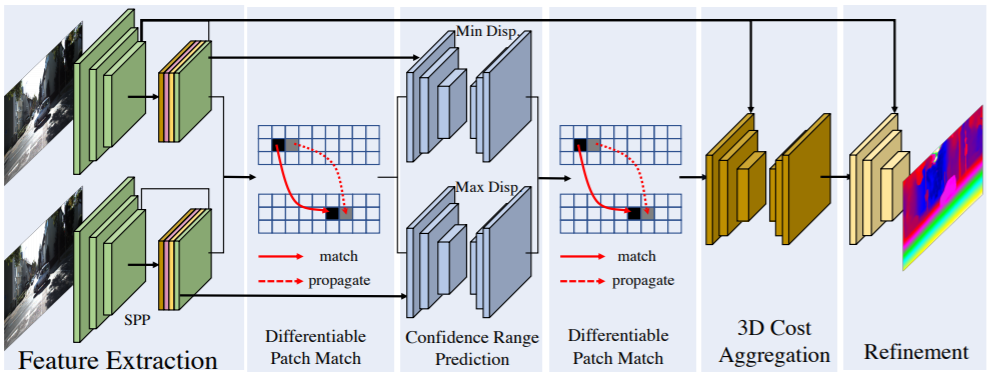
\includegraphics[width=\columnwidth]{Figure1.png}}
\caption{High-level overview of DeepPruner, source: \citep{duggal2019deeppruner}}
\label{figure1}
\end{center}
\vskip -0.2in
\end{figure}

\subsection{DeepPruner Solution}
\label{deepprunersolution}
The DeepPruner \citep{duggal2019deeppruner} algorithm contains several other elements beyond PatchMatch \citep{barnes2009patchmatch} that improve its performance that I was unable to implement due to hardware constraints. The full DeepPruner algorithm, shown in Figure \ref{figure1}, consists of feature extraction, pruning through differentiable patch match, and cost aggregate refinement phases that are all differentiable allowing for end-to-end learning. I will first explain how the solution approach to the full DeepPruner algorithm before talking specifically about my approach.

\textbf{Feature Extraction} The DeepPruner algorithm \citep{duggal2019deeppruner} starts with a 2D convolutional neural network linked to a spatial pyramid pooling module that utilizes shared parameters to create a feature volume representation for every pixel in the left image and the right image. By using residual blocks and spatial pyramid pooling the pre-processing phase can extract global feature information without losing resolution. The design of this CNN pre-processing phase is out of the scope of this paper but was modeled off of the following papers.

\textbf{Differentiable Patch Match} As discussed in Section \ref{patchmatch}, PatchMatch \citep{barnes2009patchmatch} was a pivotal algorithm used to quickly locate approximate near neighbor patches within an image or between two images. However, PatchMatch as it was originally presented in 2006 relies on many random offset probes used in the random search phase which can be computationally burdensome, and it determines which offsets to push forward by utilizing the non-differentiable \textit{arg max} algorithm.

DeepPruner \citep{duggal2019deeppruner} presents a differentiable version of PatchMatch \citep{barnes2009patchmatch} that removes the random search phase and replaces the \textit{arg max} function with the soft version to maintain differentiability. Also, in the propagation phase instead of alternating propagation from top left to the bottom right and from the bottom right to top left, the differentiable PatchMatch algorithm presented by Duggal et al. \citep{duggal2019deeppruner} utilizes one-hot filter banks for all four surrounding pixels (Figure \ref{figure2}).

\textbf{Confidence Range Prediction} The confidence range prediction phase of the DeepPruner \citep{duggal2019deeppruner} algorithm exploits a convolutional encoder-decoder network structure to narrow the search range of likely disparities for each patch. The network takes the density estimations from the initialization and propagation phase of the differentiable patch match layer and produces a confidence range of disparities, \textit{R\textsubscript{i}} = [\textit{l\textsubscript{i}}, \textit{u\textsubscript{i}}], for each pixel \textit{i}.

\textbf{3D Cost Aggregation} Using the reduced disparity range produced by the confidence range prediction layer, a 3D cost analysis is done on every disparity and the soft \textit{arg max} algorithm again used to evaluate the best disparity.

\textbf{Refinement} In the refining layer, the best disparity values for each pixel are passed into a “lightweight fully convolutional refinement network” \citep{duggal2019deeppruner} that improves the performance of the algorithm by also considering the feature information extracted by the first layer of the algorithm.  This layer serves to reduce noise within objects that may be smooth or contain repeated patterns.
\begin{figure}[ht]
\vskip 0.0in
\begin{center}
\centerline{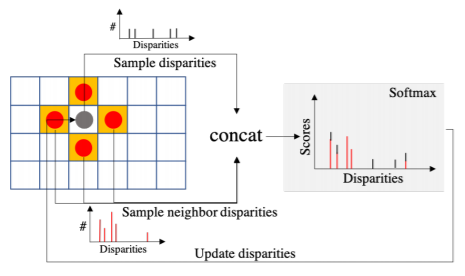
\includegraphics[width=\columnwidth]{Figure2.png}}
\caption{DeepPruner's differentiable PatchMatch, source: \citep{duggal2019deeppruner}}
\label{figure2}
\end{center}
\vskip -0.2in
\end{figure}

\subsection{My Solution}
\label{mysolution}
The first assumption I made was that the stereo images being fed into the algorithm have been rectified through preprocessing that have normalized their colors and aligned objects along the vertical plane. This important assumption greatly reduces the cost volume of my algorithm by reducing the disparity range to a 3D array along the same row of any given pixel.

Disparities for each pixel in the left image are chosen by locating the cost-minimizing disparity between a 7x7 pixel patch surrounding the pixel and corresponding pixel patches in the right image within the disparity range. For example, the cost distance function, \textit{f}(\textit{A}, \textit{B}), between patch \textit{A} in the left image and patch \textit{B} in the right image is calculated by doing a simple sum of squares between the pixel information in each of the two patches.

\textbf{Initialization} In the initialization phase I start by running a convolutional pooling algorithm on each image to initialize what will be considered the patch for each pixel. Then, for each patch in the left image, a random offset between zero and the maximum disparity uniformly.

\textbf{Propagation} During each iteration, good guesses from the initialization or random search phase are propagated to each pixel’s right and bottom neighbor (or top and left neighbor for even iterations). Each of the three disparities is translated into right image patches and run through a negative log sum of squared differences (SSD) cost function with the left patch. The \textit{arg max} function is used to assign the new lowest-cost disparity.

\textbf{Random Search} The random search phase operates similarly to the propagation phase, but instead of using neighboring offsets a random offset is selected and compared to the current offset within a decreasing radius around the current best disparity. For this algorithm, I started with a disparity range of 100 that is halved after each random search. However, after running several tests I came to the same conclusion that Duggal et al. \citep{duggal2019deeppruner} did, that the random search phase is computationally burdensome and that most patches converge without it. Instead of removing the random search phase entirely, as Duggal et al., I still preserved one random search across the entire disparity range of 100 for each iteration to cut down on runtime while still maintaining the ability to escape local minima.

\section{Implementation}
\label{implementation}
The following will describe in detail how I implemented my stereo depth estimation algorithm using differentiable PatchMatch. The algorithm was written in Python 3.8 and utilizes Numpy 1.17.3 and Matplotlib 3.0.2. The algorithm begins by pooling each image into pixel patches and initializing random offsets for each patch in the left image. Then during each of the \textit{k} iterations of the training phase, a nested loop will propagate and random search for every patch in the left image.

\textbf{Initialization} The convolutional pooling algorithm described in the previous section is done through the \textit{getPatches} function. The function takes one argument, an image as a 3D numpy array, and returns a 5D numpy array that contains a 7x7 pool of the pixels surrounding each given pixel in place of the pixel. This is done through iterating through every pixel in the image with nested loops and pooling its neighboring pixels.

Initial offsets are set by calling the function initialize offsets. This function returns a numpy array of the same height and width of the right and left images with random offsets uniformly distributed between 0 and the maximum disparity of 100. Offsets are initialized via the numpy random module using the randint function. The array used to cache the current cost or distance values for each offset is also initialized at the beginning with the same shape as the offset array and each value is calculated using the cost function.

\textbf{Propagation} The propagation phase is implemented for each pixel by applying the accepted offset for the patch above and the patch to the left and comparing the two costs to the currently accepted offset for the pixel. The simple \textit{arg max} function is called to determine which of the three offsets would remain for the patch. By considering accepted offsets above and to the left of a given patch, good offsets are effectively propagated down and to the right.

However, for odd iterations, the pixels are looped through in reverse order, from the bottom right to the top left. This gives the chance for good offsets in the lower right corners of objects to be propagated throughout the object. To implement this function the propagate patch function is split into two separate functions, propagate up and propagate down for even and odd iterations respectively.

\textbf{Random Search} As mentioned in Section \ref{implementation}, for the random search phase I simply chose offsets for each pixel patch distributed randomly across the entire disparity range. I initialized random offsets by calling the same function used to initialize the offsets at the beginning of the program outside of the patch loop to cut down on the number of times numpy \textit{randint} was called. For each patch, its currently accepted offset’s cost was compared to the new randomly selected offset and \textit{arg max} was used again to select between the two.
\begin{figure}[ht]
\vskip 0.0in
\begin{center}
\centerline{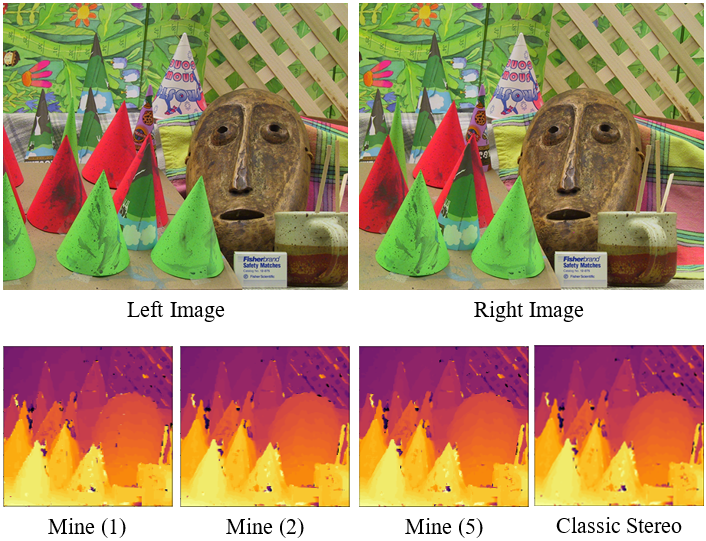
\includegraphics[width=\columnwidth]{Experiment.png}}
\caption{Disparity mapping of the Classical Stereo algorithm and my algorithm after 1, 2, and 5 iterations}
\label{experiment}
\end{center}
\vskip -0.2in
\end{figure}
\section{Evaluation / Experiments}
\label{evaluation}
The goal of my algorithm was to implement the notable PatchMatch \citep{barnes2009patchmatch} algorithm across a pair of stereo images, similar to the work done in DeepPruner \citep{duggal2019deeppruner}. What makes the PatchMatch algorithm significant is its ability to prune the search space of possible disparities for a given patch through its random search phase and its ability to propagate good guesses to neighboring patches. By reducing the search range of disparities, the runtime can be greatly reduced, varying based on the number of iterations performed by the algorithm.

To test the efficacy of my algorithm I implemented two similar algorithms, one algorithm that would perform a cost-minimization over the entire range of possible disparities for each pixel and a second algorithm that would scan the range of possible disparities using the PatchMatch algorithm described in Section \ref{implementation}. Runtimes were compared using the built-in Python Time module and the disparity maps were compared visually (Figure \ref{experiment}).

It did not make sense to compare my algorithm’s runtime with any previous works or the DeepPruner algorithm because not only was my algorithm a greatly simplified version of DeepPruner, but my algorithm was also being tested on a CPU. In the future, more extensive testing can be done with improved hardware and more components of the DeepPruner design integrated into my model.

The results of my experiment showed that for a set of images from the \textit{SceneFlow} \citep{mayer2016large} sample dataset, my algorithm was able to greatly outperform the classical stereo depth algorithm in terms of runtime while quickly converging for the majority of patches within the first few iterations. Average runtimes can be seen in Table \ref{table} and the disparity maps are shown in Figure \ref{experiment}.

\begin{table}[t]
\label{table}
\vskip 0.02in
\begin{center}
\begin{small}
\begin{sc}
\begin{tabular}{lcccr}
\toprule
\textbf{Algorithm} & \textbf{Avg. Runtime (sec.)} \\
\midrule
Classic Stereo & 506.17 \\
Patch Match (1) & 36.42 \\
Patch Match (2) & 64.88 \\
Patch Match (5) & 122.09 \\
\bottomrule
\end{tabular}
\end{sc}
\end{small}
\end{center}
\vskip -0.1in
\caption{Runtime comparisons between the Classical Stereo algorithm and my algorithm after 1, 2, and 5 iterations}
\end{table}
\section{Discussion}
\label{discussion}
As shown in Section \ref{evaluation}, the results of my experiments have shown that PatchMatch \citep{barnes2009patchmatch} has the potential to significantly reduce runtime for stereo depth estimating algorithms by grossly pruning the search space for potential disparities. However, it is clear from visual inspection that using PatchMatch as a stand-alone tool to estimate disparities would produce error rates much higher than current state-of-the-art algorithms such as DeepPruner \citep{duggal2019deeppruner}. In this section, I will go over how Duggal et al. expanded upon the PatchMatch algorithm with DeepPruner and how these expansions could have improved upon the results I saw in my experiments.

To begin, DeepPruner \citep{duggal2019deeppruner} implemented a differentiable version of PatchMatch \citep{barnes2009patchmatch} that allowed their model to take advantage of end-to-end learning. Duggal et al. took advantage of the large and diverse \textit{SceneFlow} \citep{mayer2016large} and \textit{KITTI 2015} \citep{geiger2012we} datasets to train their model with a cost function that compared their disparities directly against known disparity values. Doing so gave DeepPruner the ability to gain insights beyond just the simple SSD between neighboring pixels.

Another significant advantage to DeepPruner \citep{duggal2019deeppruner} is the feature extraction network layer implemented on both images during the pre-processing phase. There are several points within all four of the disparity maps produced in Section \ref{evaluation} (Figure \ref{experiment}) where there seem to be discontinuous disparity estimations on a single surface. The disparity estimations on the flat surface of the box in the front of the scene are clear examples of this. Had the patches of this area of the image had the global context of knowing that they all existed within the same feature, an element of voting or averaging could be done between patches to result in a more continuous estimation.

Finally, Duggal et al. \citep{duggal2019deeppruner} used their version of differentiable PatchMatch \citep{barnes2009patchmatch}, as the DeepPruner name implies, like a pruning method for narrowing the search field of likely disparity values. However, the DeepPruner algorithm later performs a 3D cost aggregation across the entirety of these disparity ranges that allows for a finer tuned output.

\section{Conclusion}
\label{conclusion}
The purpose of this paper was to review a few methods of generating disparity maps between sets of stereo images and to evaluate the effectiveness of using PatchMatch \citep{barnes2009patchmatch} to prune disparity ranges between stereo images. When compared to the classic stereo algorithm approach of searching over all possible disparities, my algorithm implementing PatchMatch was able to cut down runtime by a magnitude of 5 without any significant decrease in disparity estimation.

Although the results of my experiments showed much promise for the use of PatchMatch \citep{barnes2009patchmatch} into stereo depth estimating algorithms to cut down on runtime, more research still needs to be done to implement and test the feasibility of integrating PatchMatch into various forms of deep learning algorithms such as DeepPruner \citep{duggal2019deeppruner}.

As a means of estimating approximate near-neighbor patches PatchMatch \citep{barnes2009patchmatch} is an effective tool, but apart from a feature extraction network or other forms of pre- and post-processing PatchMatch alone is too coarse of a method for mapping disparities than state-of-the-art algorithms such as those presented by Duggal et al. \citep{duggal2019deeppruner} and Luo et al. \citep{luo2016efficient}. A possible next step to this paper could be the integration of a spatial pyramid pooling network as a pre-processing step attached to a differentiable version of PatchMatch to create an end-to-end differentiable network that may take advantage of backward propagation. Doing so may reduce error rate amongst cases of texture-less surfaces and repeated patterns by providing each pixel patch with a more global scope.

\bibliographystyle{plain}
\bibliography{references}
\end{document}
